\documentclass[tikz,border=6pt]{standalone}
\usepackage[T1]{fontenc}
\usepackage{lmodern}
\usepackage{amsmath,amssymb}
\usetikzlibrary{arrows.meta,calc,positioning,shapes.geometric,patterns,decorations.pathmorphing,backgrounds,fit}
\definecolor{ink}{HTML}{173948}
\definecolor{flow}{HTML}{167D9A}
\definecolor{heat}{HTML}{B75A23}
\definecolor{measure}{HTML}{70518A}
\definecolor{pale}{HTML}{EAF2F5}
\definecolor{muted}{HTML}{526571}
\definecolor{green}{HTML}{2E8665}
\tikzset{every node/.style={font=\sffamily\small,text=ink},
 equipment/.style={draw=ink,line width=1pt,fill=pale,rounded corners=2pt},
 process/.style={draw=flow,line width=1.1pt,-{Latex[length=2.4mm]}},
 signal/.style={draw=measure,dashed,line width=.9pt,-{Latex[length=2mm]}},
 thermal/.style={draw=heat,line width=1.1pt,-{Latex[length=2.3mm]}},
 labelbox/.style={fill=white,inner sep=2pt,font=\sffamily\footnotesize,align=center},
 annotation/.style={font=\sffamily\footnotesize,text=muted,align=left},
 panel/.style={draw=ink!20,fill=ink!2,rounded corners=3pt,inner sep=7pt,align=left},
 sensor/.style={circle,draw=measure,fill=white,line width=.8pt,minimum size=8mm,inner sep=1pt,font=\sffamily\scriptsize,align=center},
 box/.style={equipment,minimum width=3cm,minimum height=1.2cm,align=center}}
\newcommand{\atlasheader}[2]{\node[anchor=north west,font=\sffamily\bfseries\LARGE]at(0,0){#1};\node[anchor=north west,font=\sffamily\small,text=muted]at(0,-.75){#2};\draw[ink!25](0,-1.25)--(26,-1.25);}
\newcommand{\atlasfooter}[1]{\draw[ink!25](0,-15.8)--(26,-15.8);\node[anchor=north west,annotation,text width=25.8cm]at(0,-16){#1\\Original explanatory drawing for ThermoFuzzy-PID. Source traceability: Cordeiro (UFC, 2021), documented repository equations and explicit reconstruction choices.};}

\begin{document}
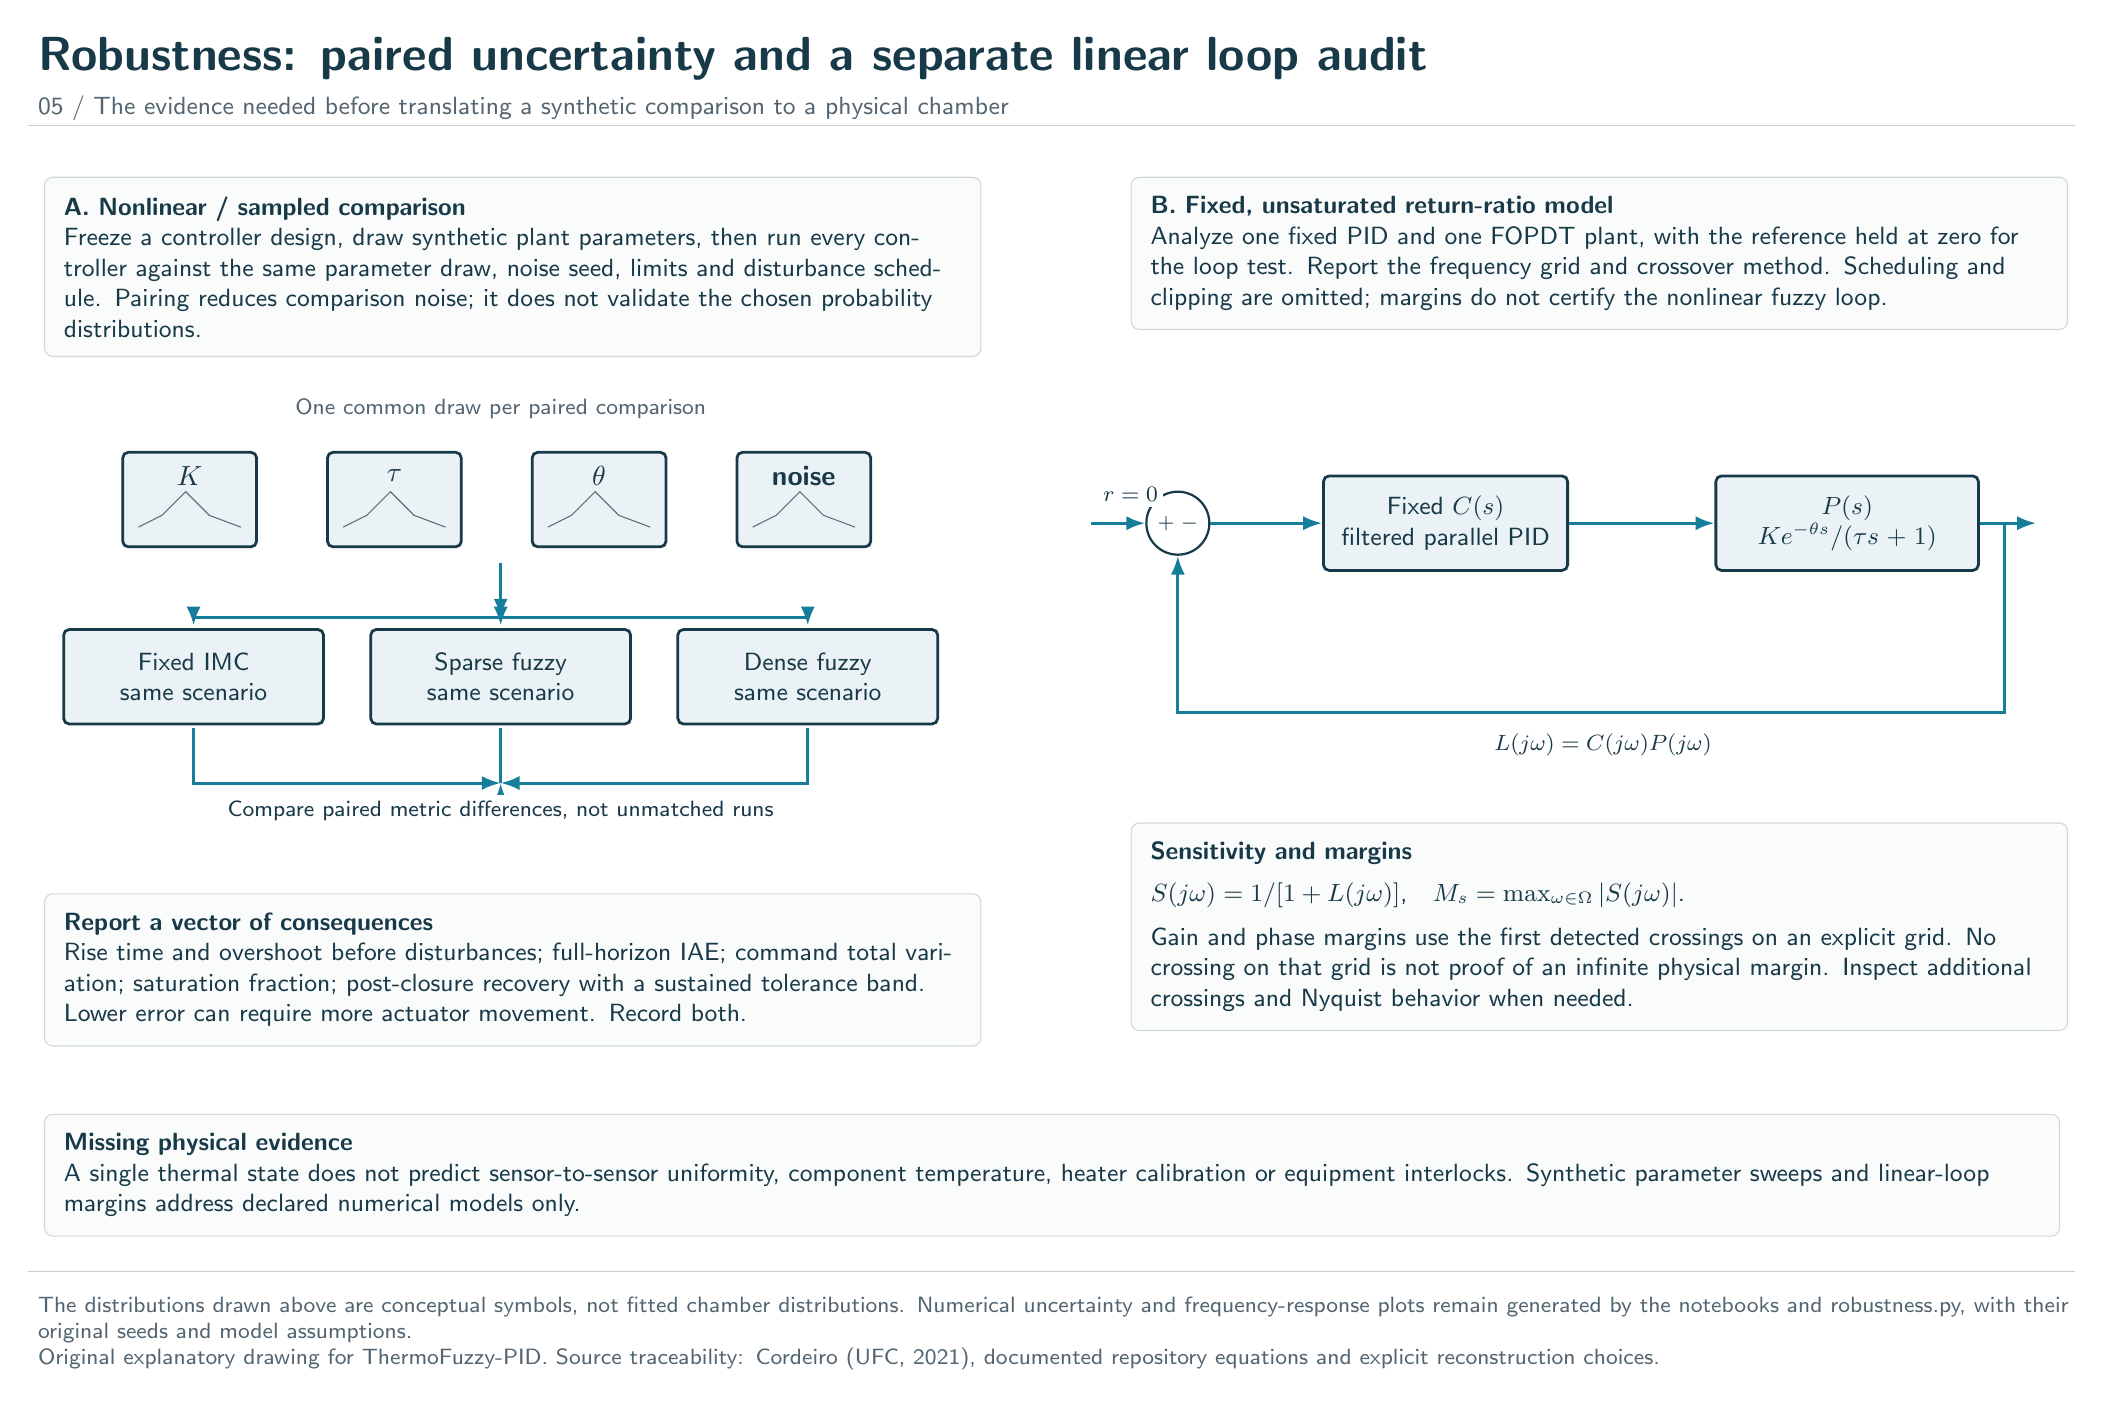
\begin{tikzpicture}[x=1cm,y=1cm]
\atlasheader{Robustness: paired uncertainty and a separate linear loop audit}{05 / The evidence needed before translating a synthetic comparison to a physical chamber}
\node[panel,anchor=north west,text width=11.4cm]at(.2,-1.9){\textbf{A. Nonlinear / sampled comparison}\\Freeze a controller design, draw synthetic plant parameters, then run every controller against the same parameter draw, noise seed, limits and disturbance schedule. Pairing reduces comparison noise; it does not validate the chosen probability distributions.};
\node[panel,anchor=north west,text width=11.4cm]at(14.0,-1.9){\textbf{B. Fixed, unsaturated return-ratio model}\\Analyze one fixed PID and one FOPDT plant, with the reference held at zero for the loop test. Report the frequency grid and crossover method. Scheduling and clipping are omitted; margins do not certify the nonlinear fuzzy loop.};
% Side-by-side physical scenario bank and continuous loop.
\foreach \x/\y/\lab in {1.2/-5.4/$K$,3.8/-5.4/$\tau$,6.4/-5.4/$\theta$,9.0/-5.4/noise}{
 \draw[equipment](\x,\y)rectangle(\x+1.7,\y-1.2);
 \node[font=\sffamily\bfseries]at(\x+.85,\y-.3){\lab};
 \draw[ink!70](\x+.2,\y-.95)--(\x+.5,\y-.8)--(\x+.8,\y-.5)--(\x+1.1,\y-.8)--(\x+1.5,\y-.95);
}
\node[annotation,anchor=south]at(6,-5.1){One common draw per paired comparison};
\draw[process](6,-6.8)--(6,-7.5);
\foreach \x/\name in {2.1/Fixed IMC,6/Sparse fuzzy,9.9/Dense fuzzy}{
 \node[box,minimum width=3.3cm,text width=2.9cm]at(\x,-8.25){\name\\same scenario};
 \draw[process](6,-7.5)--(\x,-7.5)--(\x,-7.6);
 \draw[process](\x,-8.9)--(\x,-9.6)--(6,-9.6);
}
\node[labelbox,anchor=north]at(6,-9.75){Compare paired metric differences, not unmatched runs};
\node[sensor,draw=ink] (sum)at(14.6,-6.3){$+\;-$};
\node[box,minimum width=3.1cm,text width=2.8cm] (controller)at(18.0,-6.3){Fixed $C(s)$\\filtered parallel PID};
\node[box,minimum width=3.3cm,text width=3.1cm] (plant)at(23.1,-6.3){$P(s)$\\$Ke^{-\theta s}/(\tau s+1)$};
\draw[process](13.5,-6.3)--(sum.west);
\node[labelbox,anchor=south]at(14,-6.1){$r=0$};
\draw[process](sum.east)--(controller.west);
\draw[process](controller.east)--(plant.west);
\draw[process](plant.east)--(25.5,-6.3);
\draw[process](25.1,-6.3)--(25.1,-8.7)--(14.6,-8.7)--(sum.south);
\node[labelbox,anchor=north]at(20.0,-8.9){$L(j\omega)=C(j\omega)P(j\omega)$};
\node[panel,anchor=north west,text width=11.4cm]at(14,-10.1){\textbf{Sensitivity and margins}\\[4pt]
$S(j\omega)=1/[1+L(j\omega)]$,\quad $M_s=\max_{\omega\in\Omega}|S(j\omega)|$.\\[5pt]
Gain and phase margins use the first detected crossings on an explicit grid. No crossing on that grid is not proof of an infinite physical margin. Inspect additional crossings and Nyquist behavior when needed.};
\node[panel,anchor=north west,text width=11.4cm]at(.2,-11){\textbf{Report a vector of consequences}\\Rise time and overshoot before disturbances; full-horizon IAE; command total variation; saturation fraction; post-closure recovery with a sustained tolerance band. Lower error can require more actuator movement. Record both.};
\node[panel,anchor=north west,text width=25.1cm]at(.2,-13.8){\textbf{Missing physical evidence}\\A single thermal state does not predict sensor-to-sensor uniformity, component temperature, heater calibration or equipment interlocks. Synthetic parameter sweeps and linear-loop margins address declared numerical models only.};
\atlasfooter{The distributions drawn above are conceptual symbols, not fitted chamber distributions. Numerical uncertainty and frequency-response plots remain generated by the notebooks and robustness.py, with their original seeds and model assumptions.}
\end{tikzpicture}
\end{document}
